\h{Abstract}

This book introduces Energetically Coherent Computation (ECC), a novel theoretical framework that reconceptualizes consciousness as emerging from coherent energy flows within biological systems rather than from abstract computation or symbolic manipulation. ECC represents a significant departure from traditional cognitive models by positioning consciousness as an emergent property of dynamically organized energy dynamics that span multiple scales—from molecular interactions and protein states to regional brain waves and global neural coherence. This physically grounded approach addresses fundamental challenges in cognitive science, including the symbol grounding problem, the unity of consciousness, and the relationship between physical and experiential properties.

The framework is built upon several key theoretical innovations. First, it proposes that consciousness requires specific forms of energetic coherence maintained through biological structures, particularly through astrocytic networks and the cortical neuropil. Second, it suggests that conscious states are shaped by unique transcriptomic profiles that create region-specific "alphabets" of possible energetic configurations. Third, it introduces the concept of "neural light cones" that define the causal boundaries of conscious integration. These elements work together to create a dynamically stable, unified field of consciousness that remains coherent while adapting to changing conditions.

\begin{figure}[h]
    \centering
    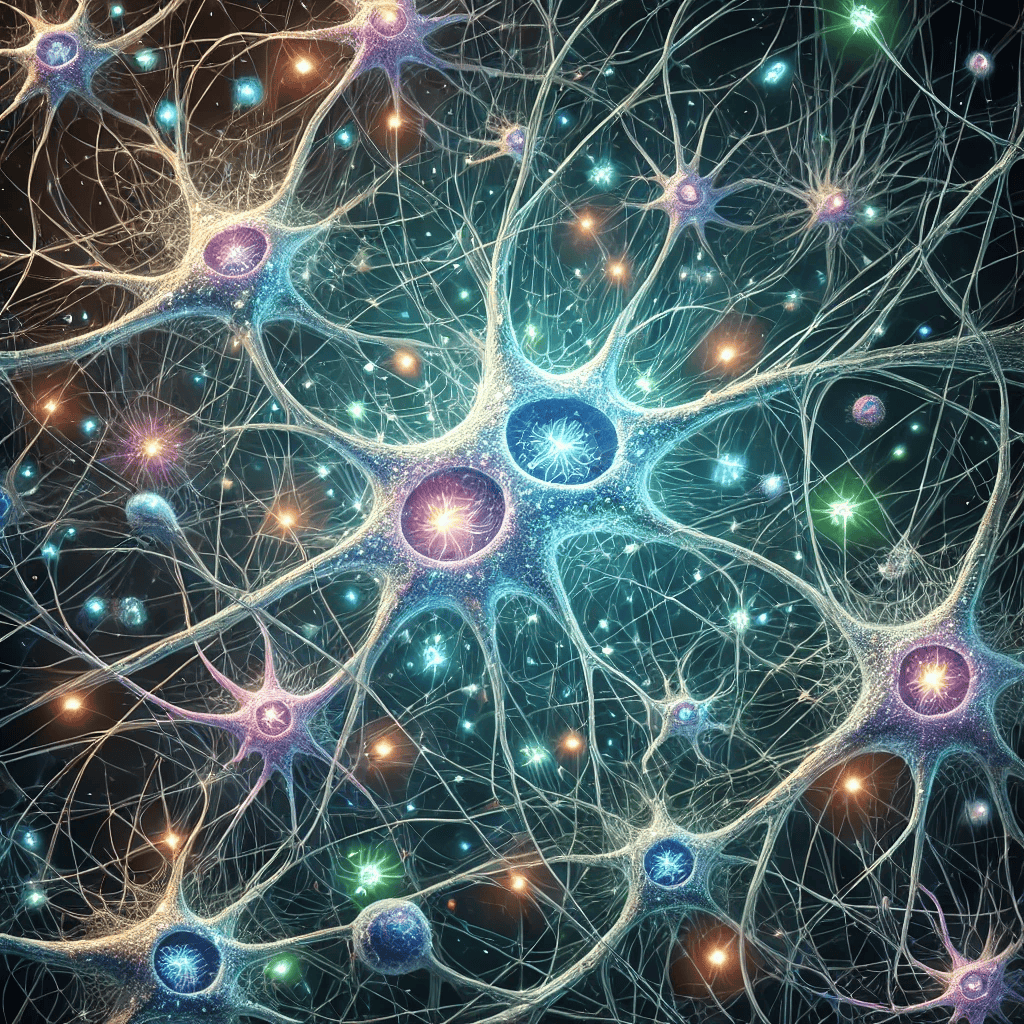
\includegraphics[width=0.8\textwidth]{astrocytes.png}

    \caption{Astrocytic Syncytia}
\end{figure}

Mathematically, ECC employs sophisticated formal tools to describe how local energy dynamics integrate into global conscious states. These include sheaf theory for modeling local-to-global coherence, the Jacobian of the stress-energy tensor for analyzing energy flows and their interactions, and principles of mutual recursion and triangulation for maintaining stability across scales. The framework also incorporates thermal noise as a boundary condition that shapes the scope and structure of conscious states, suggesting how background energy fluctuations contribute to conscious experience.

The theory offers novel interpretations of various psychological phenomena. It frames free will as the direct experience of enacting change through coherent energy flows, explains abstract thinking as a special case of conscious processing that requires active maintenance of ungrounded placeholders, and reinterprets perceptual phenomena like visual snow as manifestations of fundamental energy dynamics. Additionally, ECC provides insights into the nature of emotions, pain, and other subjective experiences by grounding them in specific patterns of energetic coherence.

ECC has significant implications for multiple fields, including neuroscience, artificial intelligence, philosophy of mind, and even anthropology. It suggests specific requirements for consciousness that go beyond computation alone, indicating why consciousness might be limited to biological systems or specially designed artificial systems that can achieve similar forms of energetic coherence. The framework also offers testable predictions about the relationship between energy dynamics and conscious experience, particularly through research on brain organoids and neuromorphic computing.

Through its integration of physical, biological, and mathematical principles, ECC provides a comprehensive framework for understanding consciousness that bridges phenomenology and neuroscience. By grounding conscious experience in the physical reality of the brain's continuous, multi-layered energy flows while maintaining mathematical rigor, it offers a promising direction for future research into the foundations of consciousness. The theory's emphasis on energetic coherence and physical embodiment represents a significant contribution to ongoing debates about the nature of mind, experience, and consciousness.